\documentclass[10pt,sigconf,letterpaper,anonymous,nonacm]{acmart}

\usepackage{amsfonts} 
\usepackage{graphicx}

\graphicspath{ {./graph/} }

\title{Tempus: Probabilistic Network Latency Verifier}
\author{WIP}

\begin{document}
\begin{abstract}
    To combat problems and bugs that a given network might have, network verifiers have emerged as 
    one of the promising solutions. 
    State-of-the-art network verifiers mainly focused on evaluating qualitative properties under 
    various scenarios of network failures, such as reachability under k-link failure. 
    However, as modern networks evolved and performance need becomes more stringent -- often 
    expressed in terms of Service Level Agreement (SLA) -- there is a need to evolve network 
    verifiers to also reason about quantitative performance properties. 
    Works in quantitative network verifiers that has arose in recent years mainly focused on one 
    side of the network performance metric: bandwidth and load violation properties. 
    Questions about the other side of network performance metric, latency, were left unanswered. 

    In this work, we introduce a verifier framework, Tempus, that can answer the probability of 
    a given temporal property being true given latency distributions of individual links and 
    nodes in the network. 
    Early evaluation shows that Tempus can verify bounded reachability property -- the probability
    that the average delay of packets traversing from a source to destination node is below $T$
    time unit -- by only adding a fraction of the state exploration overhead introduced by the 
    qualitative verifier it's built upon.
\end{abstract}

\maketitle



\section{Introduction}
Modern networks consisted of various distributed protocols such as OSPF and BGP that exchange 
routing information so that a packet can reach their intended destination efficiently, even in the 
event of a component failure.
Due to their configuration intricacies however, these protocols are notoriously hard to get right. 
It is hard for a network engineer to reason about whether their configured network fulfilled some 
intended property in various possible states of the network. 
Thus, they are left between the choice of accepting the reality of Murphy's Law or getting a tool 
to help them in this task, namely, network control plane verifier.

Popular control plane verifiers, like ARC \cite{gember2016fast}, are formulated to answer 
questions about a given property deterministically. 
In other words, given a set of states of the network (e.g. $k$-link failures) the verifier are 
expected to give a yes or no answer about the property (e.g. two nodes are reachable).
While useful to some extent, this kind of models are sometimes too restrictive since network 
operators are usually able to tolerate small fraction of failure. 
For example, a given network might have an availability SLA of 99.999\%. 
This kind of probabilistic properties have been the focus of a more recent works like NetDice 
\cite{steffen2020probabilistic}.

The network property itself can also be divided into two kinds. 
Quantitative properties like reachability and loop existence, are the common properties that are 
studied by most of the existing verifiers. 
More recent work, like QARC \cite{subramanian2020detecting}, has also explored qualitative 
properties like link bandwidth violation for a given traffic.

In this work, we're exploring the other side of the network performance metric: latency. 
Certain network deployment often necessitates some latency requirement such as an ISP that has 
latency SLA \cite{Verizon} or deployments of Time-Sensitive Networking (TSN) \cite{TSN}.
We proposed a verification framework to probabilistically verify the latency property of packets 
traversing from a source to destination node under various failure scenarios, by using latency 
information of each components in the network.

\section{Overview}
To be written


\section{On Latency Modeling}
\subsection{Latency as Path Property} 
We began our study by first pondering about a basic construct: modeling the end-to-end latency of 
a single packet.
In a packet-switched network, a packet is sent from one transmiting host to one receiving host 
through the many components of the network (e.g. links, routers, firewall) and each of those 
components might introduce some latency into the packet transmission process.
Figuring out which of those components will actually introduce latency into the packet in question, 
and by how much, is the next logical step that we must figure out.

Obviously, a given packet doesn't need to visit all network components to reach its destination 
host.
A network engineer will configure the network in such a way that a packet will only need to be 
routed via a specific subset of its components.
That specific subset is dictated by two things: how those components are connected together 
(i.e. topology) and how the control plane protocols are configured to route a packet (e.g. routing 
protocol, ACL).
Based on a variety of these setups, nodes in the network will form a forwarding table to route a 
given packet appropriately.

The goal of a classical control plane verifier then, is to use this forwarding table in some 
form to verify certain properties. %TODO: examples?
However, looking at the forwarding table alone will not give us a conclusive result regarding 
which components are going to be visited by a given packet, making verification of latency 
properties less clear.
For example, the network might be configured with a load-balancing protocol in which a packet 
departing from a source host might take multiple different \textit{paths} (with certain 
probability weights) to arrive at the destination host, possibly resulting in a different 
end-to-end latency measurement.

Therefore, we argue that when it comes to analyzing end-to-end latency, a network path should be 
the primary unit of reasoning, rather than forwarding table.
By being more specific about our unit of reasoning, we could answer verification questions more 
clearly, and we could design our verifier more efficiently since we could use it to represent 
multiple different forwarding tables that shares the same path.

\subsection{Relation to Classical Verifier}
Before we analyze the latency of a given packet that propagates through a certain network 
path however, we must make sure that said path exists in the first place.
We note that latency is a property that only make sense after connectivity between two hosts 
has been established. 
In other words, if two nodes in a network aren't even functionally connected (e.g. physical 
link failure, ACL policy), then the latency between them will \textit{always} be infinite, 
making the verification task trivial.

Fortunately, there are a rich body of work in the network verification literature regarding 
functional reachability under failure. %TODO: cite
We could then design our verifier on top of an existing classical control plane verifier.
We use it to verify reachability property, and only if the reachability property is fulfilled, 
we would verify whether the latency between two hosts fulfilled some additional condition.

\subsection{Path Latency Distribution}
Up to this point, we have talked about measuring the latency of a single packet by figuring out 
its path; analyzing which exact components it has traversed through.
However, when we try to generalize this framework and ask questions about the latency of multiple 
packets, it is apparent that the path alone is not a determinative information, as the latency 
of two packets propagating through the same path might be different due to a multitude of factors.

The natural extension to the framework then, is instead of representing latency of a path with a 
single number, we instead represent it with a continuous random variable that signifies the 
possible delay that a given packet traversing through that path might have.
This random variable will have a distribution that marginalizes over all other factors other than 
the path.

We can then use this latency distribution to verify some temporal properties in a probabilistic 
manner.
For example, we could verify the probability that a packet will be delivered in under a time 
unit by taking the CDF of the distribution.

\subsection{Path Decomposition and Convolution} \label{decomposition}
The final question that we had to decide on was how do we actually model path latency distribution
based on real component measurements.
Considering the complexity of factors that might determine the path latency distribution and the 
availability of measurement data, we settle on the assumption that the path latency distribution 
is composed of multiple independent distribution that corresponds to the latency each components 
in the path might introduce.
%TODO: confirm about independence?

Since not all components in the path will introduce latency with a non-negligible value, we 
specifically choose to model two source of latency in the path's components which we deem 
significant: \textbf{link propagation latency} and \textbf{queuing latency}.
%TODO: expand on how to get the data later

Propagation delay is the latency that is introduced by the links in the network, which is 
independent of the traffic load in the system.
Queuing delay is the latency that the queuing process in the node introduced. 
Unlike propagation delay, queuing delay might be dependent on load in the system, since the more 
packets there are in the queue, the more delay the node will introduce to a subsequent packets.

For propagation delay, the semantic of this random variable is relatively straightforward: it is 
the distribution of latency that a given link will introduce.
For queuing delay however, this random variable represents the delay that a given queuing process 
will introduce, marginalized over various traffic pattern that a given network state might have 
resulted.

In order to obtain the overall path latency distribution from these per-component latency 
distributions, we do a convolution operations over all the relevant component's latency 
distributions.
Since not all distributions can be convolved in a closed-form fashion, we use a numerical 
convolution technique with a guaranteed error bound. 
We initially consider a Monte-Carlo simulation in order to approach numerical convolution, but 
the lack of a general technique to measure error made us opt for the formerly mentioned method.


\section{Encoding}
We divide the problem of latency verification into two parts: 
verifying that two nodes are reachable (\textit{functional} property) and only if 
the functional property is fulfilled, we would verify whether the latency between 
two nodes fulfilled some additional condition (\textit{temporal} property).

\subsection{Topology Graph}
For functional property verification, NetDice \cite{steffen2020probabilistic} 
has laid the way for verifying reachability between two nodes under failure in a 
probabilistic and efficient manner. 
In this framework, the physical network is encoded in an edge-labeled directed graph 
$G_t = (V_t, E_t)$ where $V_t$ represents the nodes in the network and 
$E_t$ represents the functional connectivity between a source and a destination node. 
A physical link is then represented as a pair of symmetrical edges that shares the same source 
and destination node but with opposite direction (e.g. $v_1 \rightarrow v_2$ and $v_2 
\rightarrow v_1$).

To represent the component's random failure, NetDice defined two failure rates.
The first failure rate is the chance that a given physical link in the network will go down.
The second failure rate is the chance that a given node in the network will go down.
These rates are shared between all links / nodes in the network.
Internally however, the node failure rate will be translated into the link failure rate 
with a Bayesian Network model, since a node failure can be modeled with the failure of each 
links connected to it.

We refine NetDice's model slightly by allowing each links to have different failure rate.
We label each edge in $E_t$ with a function $r: E_t \rightarrow \{x \in \mathbb{R} \mid 0 \le x 
\le 1\}$ that represents the failure rate of a given physical link.
As a consequence, two symmetrical edges (i.e. two edges that shares the same node pairs but with 
opposite direction) will also share the same failure rate, and will be disabled in a coupled 
fashion.

\subsection{Routing}
On top of this topology, NetDice also defined additional informations that would be used
by a routing protocol to determine the valid path(s) between two nodes $src, dst \in V_t$ given 
a particular link failure scenario. 
These routing informations would also be used by their optimization algorithms to reduce the 
amount of states that are going to be explored.

NetDice implemented iBGP and OSPF (with ECMP) routing protocols.
They encode the relevant routing information by assigning some labels to the vertices or edges
in the topology.
In OSPF for example, we define a function $w_{ospf}: E_t \rightarrow \mathbb{N}$ as the edge-label 
that represents the positive weight of a link.
They would later be used to compute the convergent paths of a given network state 
(\ref{verification}).

\subsection{Latency Label}
Similarly, we could also use this edge-labeling technique to represent latency. 
As mentioned in \ref{decomposition}, our model will encode two kinds of latency: link propagation 
and queuing in the node.
We will encode these latencies by equipping the model with two additional labels.

Encoding link propagation latency is fairly straightforward. 
We define a function $l_p: E_t \rightarrow \mathcal{D}$ where $\mathcal{D}$ is a set of 
continuous univariate distribution that has a minimum value of $0$.
This distribution signifies the time it would take for the respective physical link to transmit 
a packet from one end to another.
Because of this, just like $r$, two symmetrical edges will share the same distribution.

To encode node queuing latency, we first note that the queuing mechanism in modern switches 
usually resides on the output port. %TODO: Cite PISA?
Since a port in a switch is only connected to one other port, we could effectively assign the 
latency to the connectivity between switches.
To do this, we define a function $l_q: E_t \rightarrow \mathcal{D}$ where $\mathcal{D}$.
Unlike $l_p$ however, two symmetrical edges will have different distribution since they 
represent two different output queues.


\section{Verification} \label{verification}
From a labeled graph that encodes a given network, we will then do functional verification 
and temporal verification in the following way:

\subsection{Functional Verification}
For functional verification, we will essentially do the exploration technique employed by NetDice.
However, we made some modifications to the algorithm in order for it to remember and pass 
necessary informations to the next stage, which is the temporal verification.
We will describe the high-level description of NetDice's algorithm in light of our modification
as follows:

\subsubsection{Network State}
Let a network state $s_i$ be defined as a 2-tuple $(U, D)$ where $U$ is a set of links that are 
alive / up and $D$ is a set of links that are dead / down.
We then define a set $S$ that represents all possible network states in a given topology. 
Our goal is to identify a subset of $S$ where each element is a network state that can connect 
the source and destination node given a convergent behavior of a routing protocol.

This framework fits nicely with the framework of probability theory, where $S$ represents the 
sample space and the power set of $S$ represents the possible events, one of which is the one
we care about: the event that a packet from a source node can reach a destination node.
The way we assign probability to events is to simply do a summation over the product of all the 
failure and success rate of each links in the network state.

The straightforward and naive way to compute the probability of this event is to iterate over all 
the network state. 
We then determine whether that network state can fulfill said property and which path it will 
take. 
If yes, then we would compute the probability from the product of the link's failure and success 
rate, and add it to the running sum.
If no, then we could skip the computation altogether.

While natural, this brute-force algorithm is obviously doesn't scale since it will take 
$2^{|E_t|}$ iterations. 

\subsubsection{Super-state}
NetDice \cite{steffen2020probabilistic} solves this issue by noticing that we could prune over some 
states that are guaranteed not to change the convergent paths of the current network state, by 
marginalizing over \textit{cold edges}.
Said another way, we could merge multiple network states into a single super-state that shares 
the same convergent paths.

In NetDice, we start from a perfect network state (i.e. $s_i = (U, D)$ where $D = \emptyset$).
We then determine whether that network state can fulfill said property and which path it will 
take, similar to the brute-force method.
If no, then it is safe to say that the source node can never reach the destination node in all 
network state.
If yes, then we could use the logic of the routing protocol to determine the set of cold edges, 
(i.e. edges whose failure won't change the convergent paths). 
Edges that are not part of this set is called \textit{hot edges} $h_i = (U, D)$.
Instead of using $s_i$ to compute the probability of the current state, NetDice only use the set 
of hot edges to compute the probability of them being alive ($h_i = (U, D)$ where $D = \emptyset$).
This in effect computes the probability of multiple network state at once.

Next, instead of examining other network state at random, we instead iterate over the links in 
$h_i$.
By definition, if we fail a link that belongs to $h_i$, then the convergent paths will change.
To cover all of those possibilities efficiently, NetDice iterate over all the links in $h_i$, 
disabled them, re-enabled them, and move to the next edge to do the same.
If $h_i = ((e_1, e_2, ..., e_j), \emptyset)$, then we would enqueue $(\emptyset, (e_1))$, 
$((e_1), (e_2))$, $((e_1, e_2), (e_3))$, ..., $((e_1, e_2, ..., e_{j-1}), (e_j))$.
Thus, instead of exploring $2^j$ events, we will enqueue $j$ events instead. 

NetDice's exploration will effectively form a tree, where each level of the tree represents 
how many links we will explicitly put down.
The root is the event where we have empty hot edges, and the leaves are where the hot edges 
are full.

\subsubsection{Convergent Paths}
Remember instead of discarded

\subsubsection{State and Functional Path Probability}
State 

\subsection{Temporal Verification}
Since we assign each links and output queue in the network with a certain latency distribution, 
computing the probability of the temporal property involves convolving the the paths we got from 
functional verification and measuring the statistical property of the resulting distribution.
However, while NetDice has shrunk the exploration space compared to brute-force iteration, for
the purpose of temporal verification, further optimization can be done.

\subsubsection{Mega-state}
The first is what we call \textbf{hot-edges union}. 
The idea is, while each hot-edges events has the same convergent paths, it is not guaranteed to be 
unique. 
Two or more of these events can have the same convergent paths.
Therefore, we could merge these two events and compute the convolution for a given path once.

\subsubsection{Path Memoization}

% \textbf{First}, we do the functional verification with $G_t$ similar to what NetDice 
% \cite{steffen2020probabilistic} have done. 
% In addition, we also collect additional information from each state (e.g. convergent 
% paths) to be used in the temporal verification step. 

% \textbf{Second}, we compute the total path latency distribution from the convergent path(s) in each 
% state with $G_l$.
% This is done by convolving over the latency distribution of each component in the path. 
% Since not all convolutions can be calculated analytically, we implemented a numerical convolution 
% method via mixture distribution, DIRECT \cite{rover2017discrete}, which is able to convolve two 
% distribution with a KL divergence error bound.
% Multiple states can share the same convergent path(s), so \textit{only a fraction of the states need to be 
% explored}.

% \textbf{Third}, we calculate the probability of a given temporal property being true in that state. 
% For example, given a \textit{bounded reachability property} (probability of whether a packet can 
% traverse from a source to destination below some time unit $T$), we can compute its probability by 
% integrating the PDF from $0$ to $T$. 
% We then combine all of the \textit{temporal} and \textit{functional} probability in each state to 
% get the final probability: the probability of \textit{the network} fulfilling a temporal property.

% TODO: intro, reformalize graph formulation, citations
% Does a figure about topology graph and latency graph will be useful?
% Multimedia context on older networked system Klara Nahrstedts
% Graph 

\section{Evaluation}
\subsection{Scalability}

\subsubsection{States Explored}
\begin{figure}[h]
    \centering
    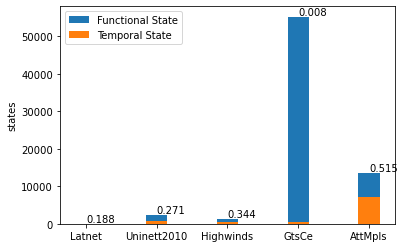
\includegraphics[scale=0.5]{states}
    \caption{States explored for temporal verification and functional verification}
    \label{fig:states}
\end{figure}

\subsubsection{Wall-clock Time}
\begin{figure}[h]
    \centering
    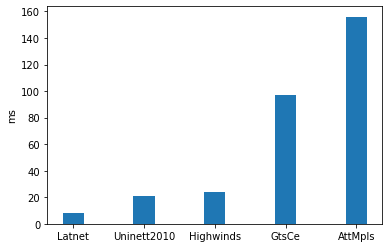
\includegraphics[scale=0.5]{wallclock}
    \caption{Time took for temporal verification}
    \label{fig:wallclock}
\end{figure}

\subsection{Optimization Effectiveness}

% On the correctness side, we want to validate whether the result of our verifier is equivalent to 
% another verifier that has lower fidelity (i.e. functional property only) if we set the temporal 
% property to be virtually unconstrained (e.g. bounded reachability with a very high $T$).

% On the performance side, we will evaluate the verifier by measuring the amount of additional 
% overhead that the temporal verifier would introduce, measured by the amount of states that 
% need to be re-explored (in the second step) and / or the amount of convolution operation performed. 
% Early result on Highwinds \cite{knight2011internet} network shows that out of 2344 states 
% produced by step 1, only 459 got re-explored on step 2.

\section{Related Works}

\section{Future Works}

\section{Conclusion}

\bibliography{cit}
\bibliographystyle{ieeetr}
\end{document}